\chapter{Arhitektura i dizajn sustava}

\section{Stil arhitekture}

	Budući da je glavna ideja bila napraviti jednostraničnu aplikaciju (engl. \textit{single page application, SPA}) i koristiti radni okvir Spring Boot,  odlučili smo se za \textbf{višeslojnu arhitekturu} (engl. \textit{multi-layer architecture}).\\\\
	\textbf{Višeslojna arhitektura} je logička nadogradnja klijent-poslužitelj arhitekture (engl. \textit{client-server architecture}).\\\\
	Arhitektura \textbf{klijent-poslužitelj} se sastoji od dva potpuno odvojena sustava.\\
	\textbf{Klijent} je računalo ili program koji dohvaća neke podatke. Te podatke mu pruža drugi program, kojeg zovemo \textbf{poslužitelj}. Poslužitelj ne pohranjuje nikakve podatke o klijentu, niti se nalazi u različitim stanjima (engl. \textit{stateless}).
	
	\begin{figure}[H]
		\centering
		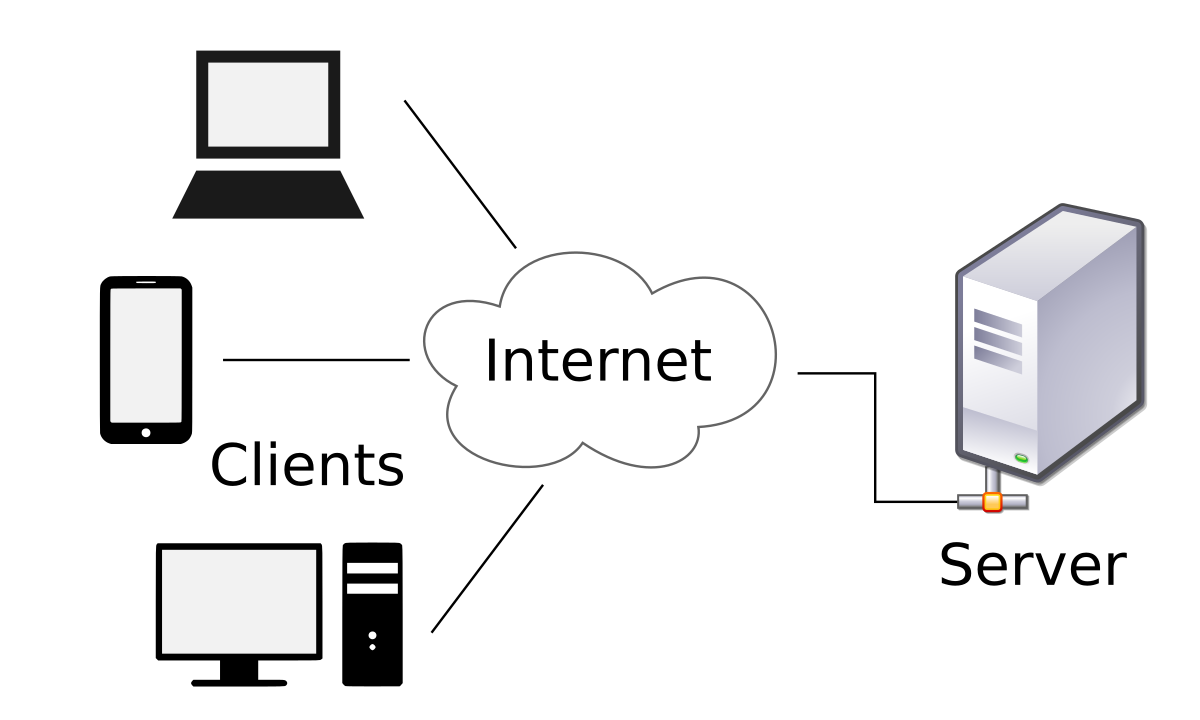
\includegraphics[width=\linewidth]{slike/client-server.png}
		\caption {Klijent-poslužitelj arhitektura,  Izvor: https://en.wikipedia.org/wiki/Client-server\_model}
		\label{fig:client-server}
	\end{figure}

	\noindent Višeslojna arhitektura također koristi načelo razdvajanja klijentske i poslužiteljske strane, ali se programska potpora sastoji od više od dva logička sloja. \\
	U našoj implementaciji, za koju ćemo koristi radni okvir (engl. \textit{framework}) \textbf{Spring Boot} i knjižnicu (engl. \textit{library}) \textbf{React}, višeslojna arhitektura će imati 6 slojeva: 
	\begin{enumerate}
		\item \textbf{sloj korisničke strane}  
		\begin{itemize}
			\item Sloj koji je izravno vidljiv korisniku, preko njega korisnik koristi aplikaciju. U pozadini se koristi Javascript kojim se šalju zahtjevi i primaju odgovori u JSON formatu.
			\item Pripada klijentskoj strani.
		\end{itemize}
		
		
		\item \textbf{sloj nadglednika} (engl. \textit{controller}) 
		\begin{itemize}
			\item Prvi sloj na poslužiteljskoj strani.
			\item Prihvaća zahtjeve i poslovnu logiku prosljeđuje sloju usluge tj. servisima za obradu. Vraća na klijentsku stranu podatke koje sloj usluge pripremi za njega.
		\end{itemize}
		
		\item \textbf{sloj usluge} (engl. \textit{service})
		\begin{itemize}
			\item Sloj koji obavlja poslovnu logiku i u svojem radu često komunicira sa slojem za pristup podatcima.
		\end{itemize}
		
		\item \textbf{sloj za pristup podatcima} (engl. \textit{data access object, DAO})
		\begin{itemize}
			\item Sloj kojeg servisi(sloj usluge) koriste za komunikaciju s bazom podataka (dohvat, spremanje).
		\end{itemize}
		
		\item \textbf{sloj domene} (engl. \textit{domain})
		\begin{itemize}
			\item Model baze podataka predočen u programski kod, predstavlja podatke kojima DAO pristupa.
		\end{itemize}
		
		\item \textbf{sloj baze podataka} 
		\begin{itemize}
			\item Sloj koji služi stvarnom spremanju u bazu podataka. 
			\item Interna Spring Boot implementacija, nije dio implementacije našeg razvojnog tima. 
		\end{itemize}
		
	\end{enumerate}

	\begin{figure}[H]
		\centering
		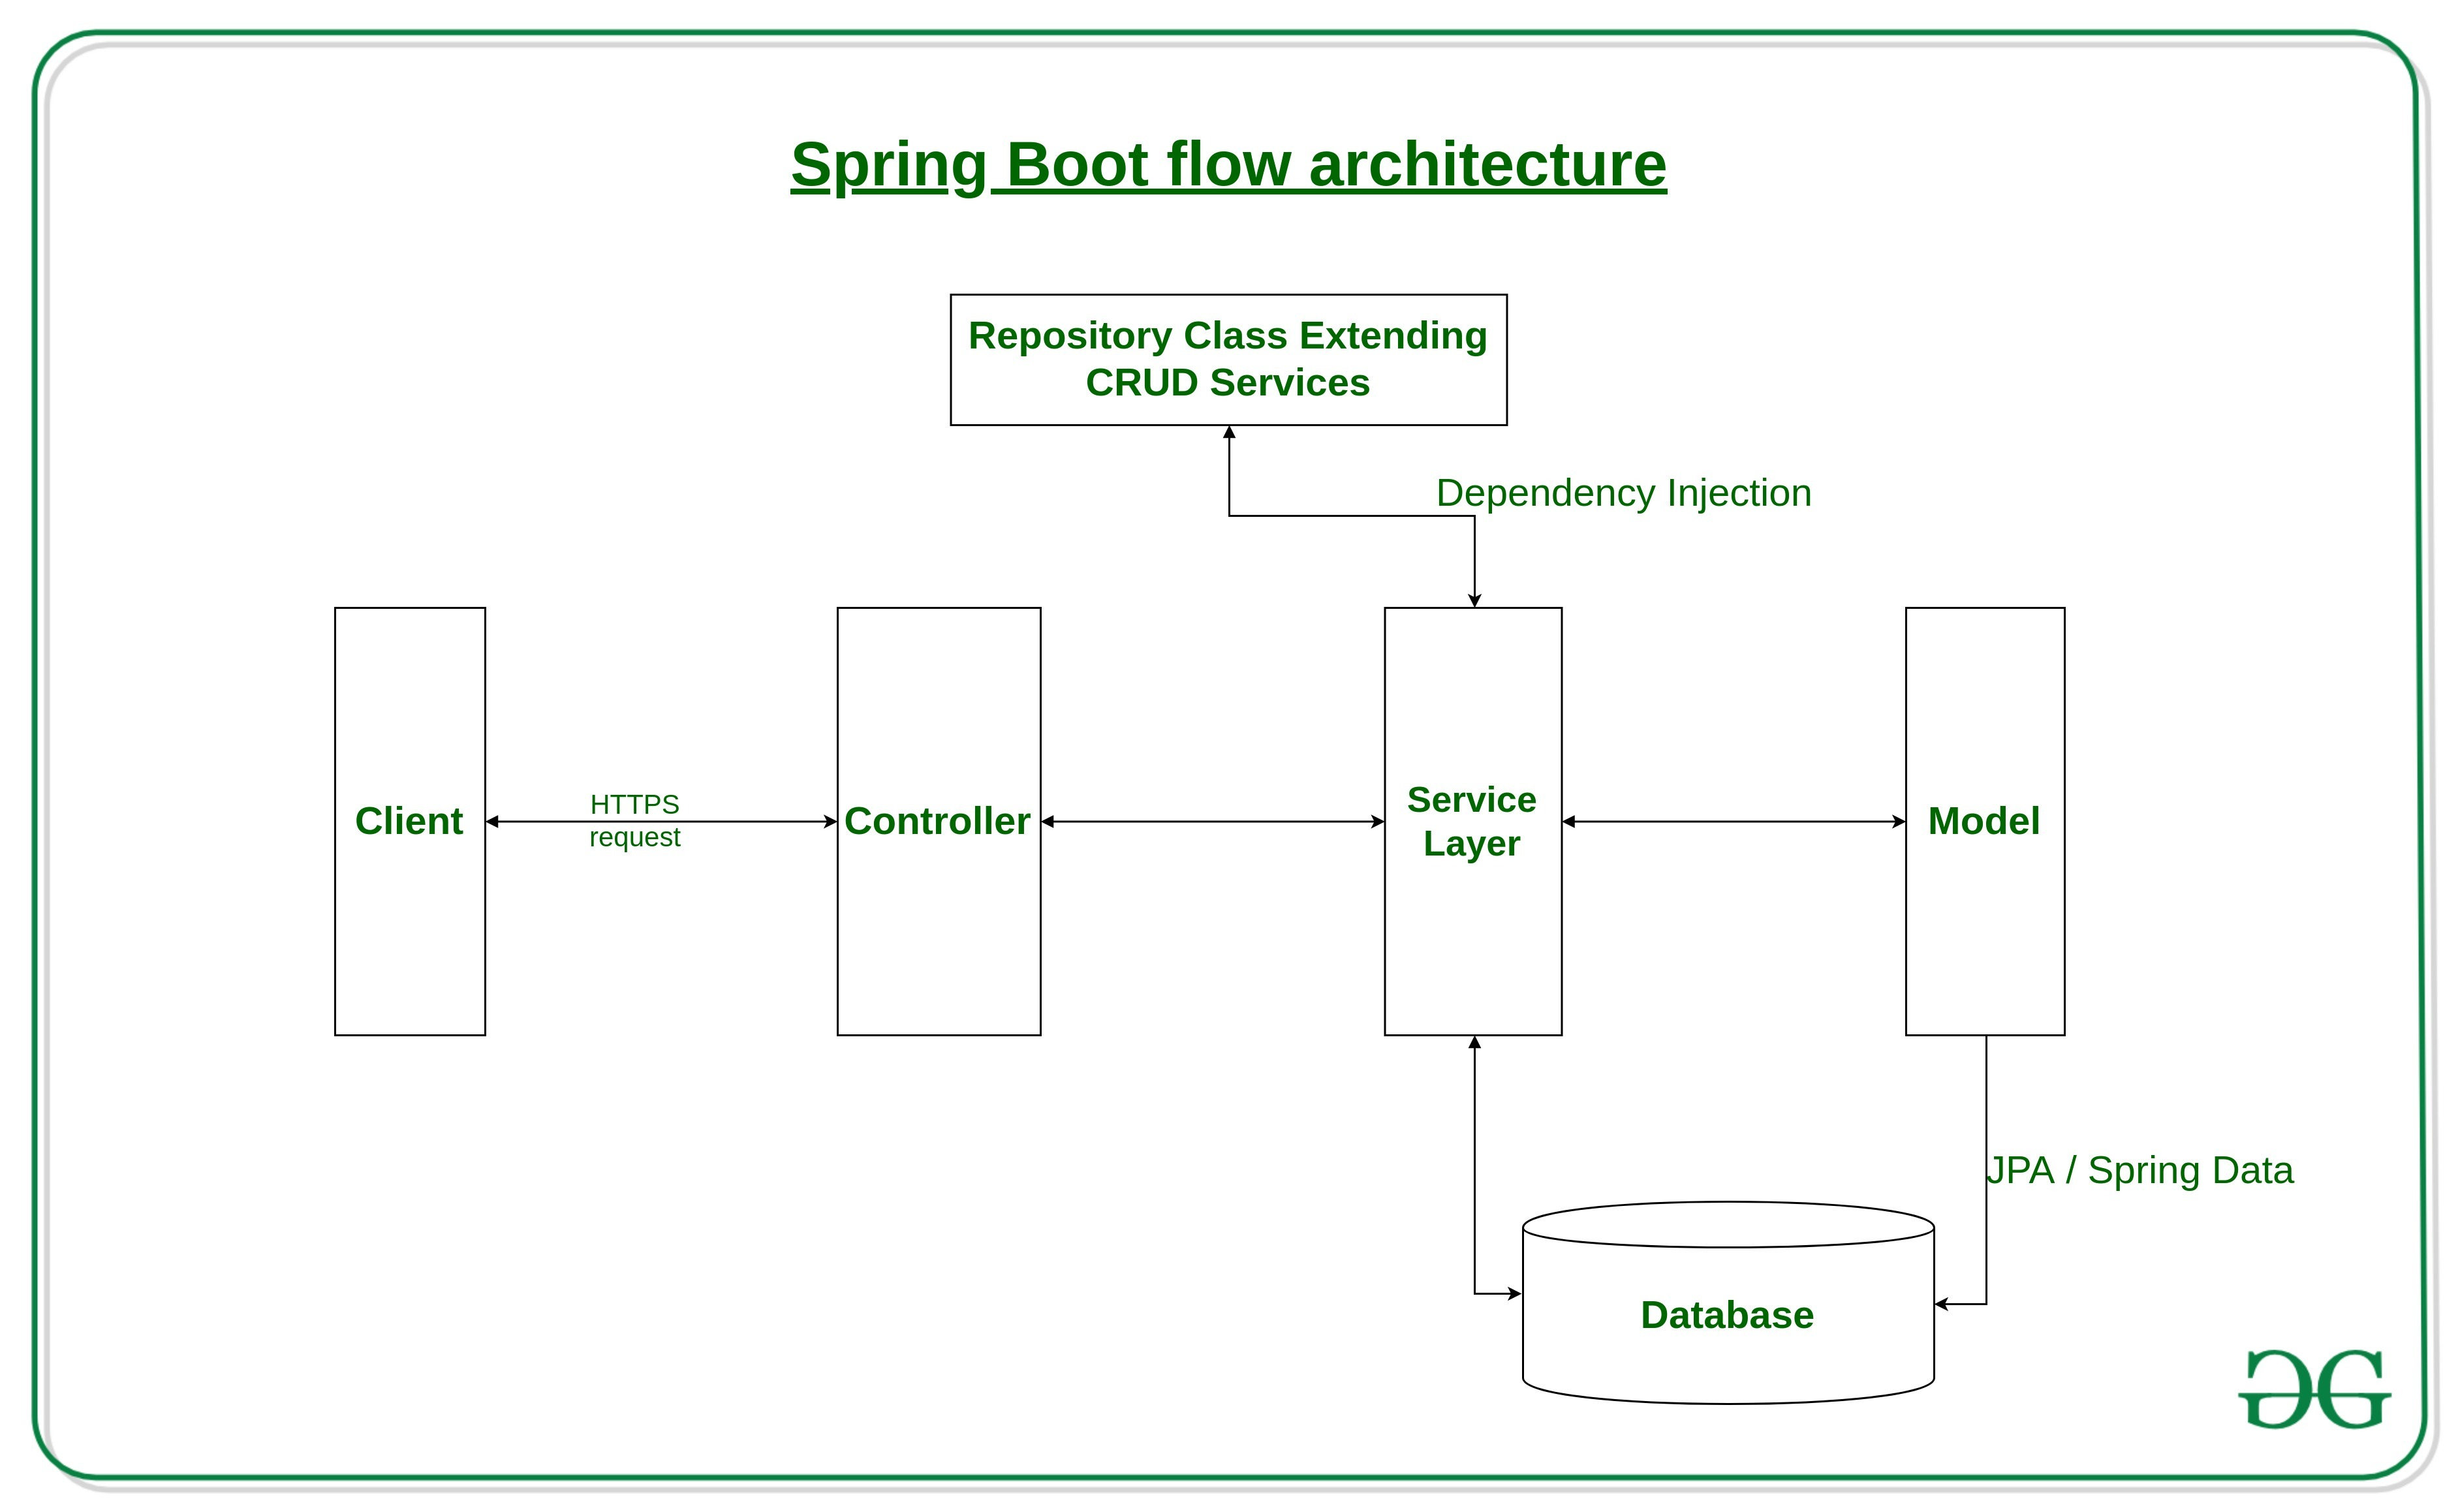
\includegraphics[width=\linewidth]{slike/spring-boot-layers.jpg}
		\caption {Spring Boot višeslojna arhitektura, Izvor: https://www.geeksforgeeks.org/introduction-to-spring-boot
		}
		\label{fig:spring-layers}
	\end{figure}

\newpage
	\subsection{Backend}
		Za razvoj backend dijela aplikacije se koristi Java programski jezik s radnim okvirom \textbf{Spring Boot} sa svojim podsustavima (Spring Web, Spring Data, Spring Security). Spring Boot pruža odličnu podršku za razvoj višeslojne aplikacije.
		
		\begin{figure}[H]
			\centering
			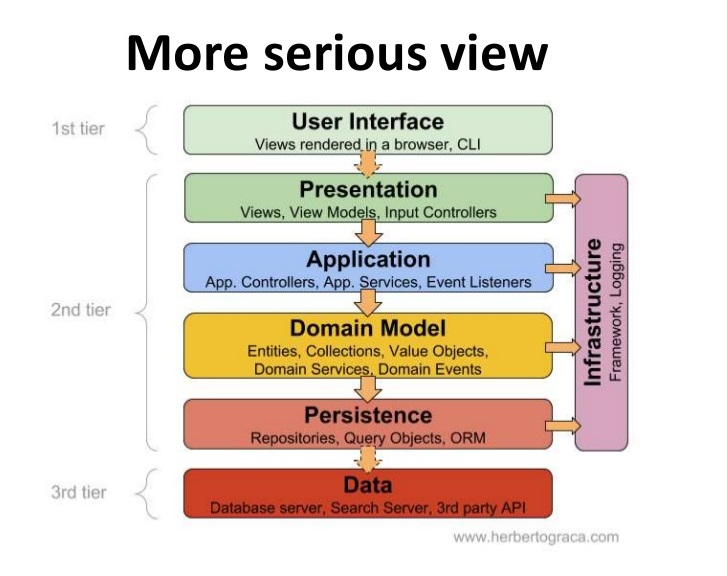
\includegraphics[width=\linewidth]{slike/spring-6-layers.jpg}
			\caption {Spring Boot - 6 slojeva arhitekture, Izvor: https://www.slideshare.net/alimenkou/hexagonal-architecture-with-spring-boot-136745841
			}
			\label{fig:spring-6-layers}
		\end{figure}
		
		
	\subsection{Frontend}
		Za razvoj frontend dijela aplikacije se koristi knjižnica \textbf{React} koja olakšava izradu komponenti za prikaz korisničkog sučelja te omogućava razvoj SPA (engl. \textit{single page application}). Komponente će se graditi s \textbf{HTML}-om (Hypertext Markup Language) te oblikovati s \textbf{CSS}-om (Cascading Style Sheets). Osim vlastitog oblikovanja koristit će se CSS radni okvir \textbf{Bootstrap} koji ima velik izbor već uređenih komponenti.
		

		

	\newpage	
		\section{Baza podataka}
			
			
		Za potrebe ove baze koristit ćemo sljedeće entitete:
			\begin{itemize}
				\item korisnik
				\item uloga
				\item obrazac\_odgovor
				\item obrazac\_korisnik
				\item obrazac\_vrsta
				\item resurs
				\item lokacija
				\item odvoz\_lokacija
				\item odvoz
				\item odlagalište
				\item otpad\_vrsta
				\item proizvod
			\end{itemize}
		Odlučili smo se za relacijsku bazu podataka koja sadrži entitete i atribute zbog lakše prilagodbe stvarnom svijetu. Kod naše baze svaki entitet će kao primarni ključ sadržavati ID koji će se pri unosu novih podataka automatski povećavati.
		
			\subsection{Opis tablica}
			
				\textbf{Korisnik}
					Entitet sadrži atribut ID koji je primarni ključ, a uz njega sadrži i atribute korisničko\_ime, lozinka, ime, prezime, lokacija\_id, email adresa i uloga\_id. Atribute korisničko\_ime i lozinka korisnik sam određuje i tu kombinaciju imena i lozinke koristi za login na stranicu. Osim podataka koji su potrebni za login korisnik ako ima ulogu Građanin također unosi i svoje osobne podatke koji se spremaju na mjesto ostalih atributa dok kod uloge Zaposlenik ti atributi se postavljaju na NULL. Entitet korisnik vezan je s entitetima uloga, obrazac\_odgovor, korisnikov\_obrazac i lokacija. S entitetom uloga je vezan vezom Many-to-One gdje se uloga\_id referencira na atribut ID kod entiteta uloga jer korisnik može imati samo jednu ulogu dok se ista uloga može dodijeliti više korisnika. Preko veze s entitetom lokacija koja je One-to-One jer korisnik može imati samo jednu adresu stanovanja, a jedna adresa može biti dodijeljena samo jednom korisniku, dobivamo adresu stanovanja korisnika. Ovisno o ulozi koja je dodijeljena korisniku on može biti povezan s još 2 entiteta preko svojeg ID-a, a ti entiteti su obrazac\_odgovor i obrazac\_korisnik, a veza je opisana kod ta dva entiteta.
				
				
				\begin{longtabu} to \textwidth {|X[6, l]|X[5, l]|X[10, l]|X[10, l]|}
					
					\hline \multicolumn{4}{|c|}{\textbf{korisnik}}	 \\[3pt] \hline
					\endfirsthead
					
					\hline \multicolumn{4}{|c|}{\textbf{korisnik}}	 \\[3pt] \hline
					\endhead
					
					\hline 
					\endlastfoot
					
					\cellcolor{LightGreen}ID & INT	&  	 jedinstveni identifikator & primarni ključ, increment	\\ \hline
					korisnicko\_ime	& VARCHAR &   ime koje je korisnik izabrao za login & not null, unique	\\ \hline 
					lozinka & VARCHAR &   hash lozinke & not null\\ \hline 
					ime & VARCHAR	&  	ime građanina &	\\ \hline
					prezime & VARCHAR	&  	prezime građanina &	\\ \hline
					lokacija\_id & INT	&  	ID lokacije koji određuje adresu korisnika & unique, strani ključ->lokacija.ID	\\ \hline 
					email adresa & VARCHAR & email adresa građanina & unique\\ \hline 
					\cellcolor{LightBlue} 	uloga\_id & INT & ID uloge koja je dodijeljena korisniku &unique, \newline strani ključ->uloga.ID\\ \hline 
					
					
				\end{longtabu}
				\textbf{Uloga} 
					Entitet sadrži atribut ID koji je primarni ključ i pomoću njega se povezuje s entitetom korisnik, a uz njega ima i atribut naziv koji poprima vrijednost mogućih uloga. 
				
				\begin{longtabu} to \textwidth {|X[6, l]|X[6, l]|X[10, l]|X[6, l]|}
					
					\hline \multicolumn{4}{|c|}{\textbf{uloga}}	 \\[3pt] \hline
					\endfirsthead
					
					\hline \multicolumn{4}{|c|}{\textbf{uloga}}	 \\[3pt] \hline
					\endhead
					
					\hline 
					\endlastfoot
					
					\cellcolor{LightGreen}ID & INT	&  	 jedinstveni identifikator & primarni ključ, increment	\\ \hline
					naziv	& VARCHAR &   dodijeljena uloga	& unique \\ \hline 
				\end{longtabu}
			
				\textbf{Obrazac\_korisnik} 
					Osim primarnog ključa entitet sadrži atribute naslov, korisnik\_id, opis, vrsta\_id, resurs\_id, resurs\_količina. Atribut naslov označava o čemu je obrazac, dok atribut opis sadržava detaljni opis što korisnik želi. Entitet je povezan s entitetom korisnik preko korisnik\_id-a i to vezom Many-to-One jer jedan korisnik može napraviti više obrazaca dok jedan obrazac može pripadati samo jednom korisniku. Osim što je vezan s entitetom korisnik, entitet se također povezuje s entitetima obrazac\_vrsta i resurs preko iste veze, a to je Many-to-One jer jedan resurs ili obrazac\_vrsta može pripadati više različitih obrazaca\_korisnik.
				
				\begin{longtabu} to \textwidth {|X[7, l]|X[6, l]|X[10, l]|X[15, l]|}
					
					\hline \multicolumn{4}{|c|}{\textbf{obrazac\_korisnik}}	 \\[3pt] \hline
					\endfirsthead
					
					\hline \multicolumn{4}{|c|}{\textbf{obrazac\_korisnik}}	 \\[3pt] \hline
					\endhead
					
					\hline 
					\endlastfoot
					
					\cellcolor{LightGreen}ID & INT	&  	 jedinstveni identifikator & primarni ključ, increment	\\ \hline
					naslov	& VARCHAR &   naslov obrasca  &not null	\\ \hline 
					\cellcolor{LightBlue}korisnik\_id	& INT &   ID korisnika koji je kreirao obrazac\_korisnik	 &not null, strani ključ->korisnik.ID\\ \hline 
					opis	& TEXT &   detaljan opis što korisnik želi dobiti obrascem	& not null\\ \hline 
					\cellcolor{LightBlue}vrsta\_id	& INT &   određuje tip obrasca	& not null, strani \newline ključ->obrazac\_vrsta.ID\\ \hline 
					\cellcolor{LightBlue}resurs\_id	& INT &   određuje tip resursa &strani ključ->resurs.ID	\\ \hline 
					resurs\_količina	& INT &   broj koliko korisnik želi resursa	&not null ako resurs\_id nije null\\ \hline 
				\end{longtabu}
			
				\textbf{Obrazac\_odgovor} 
				Entitet osim primarnog ključa sadrži atribute \newline obrazac\_korisnik\_id, korisnik\_id i sadržaj. Pomoću atributa obrazac\_korisnik\_id povezuje se s entitetom obrazac\_korisnik vezom One-to-One tj. jedan obrazac\_odgovor pripada jednom obrascu\_korisnik i obrnuto. Također je povezan s entitetom korisnik sa korisnik\_id vezom Many-to-One jer jedan korisnik može napraviti više obrazaca\_odgovor dok jedan obrazac može biti kreiran od točno jednog korisnika. Zadnji atribut sadržaj sadrži odgovor na neki obrazac\_korisnik.
				
				\begin{longtabu} to \textwidth {|X[12, l]|X[3, l]|X[14, l]|X[16, l]|}
					
					\hline \multicolumn{4}{|c|}{\textbf{obrazac\_odgovor}}	 \\[3pt] \hline
					\endfirsthead
					
					\hline \multicolumn{4}{|c|}{\textbf{obrazac\_odgovor}}	 \\[3pt] \hline
					\endhead
					
					\hline 
					\endlastfoot
					
					\cellcolor{LightGreen}ID & INT	&  	 jedinstveni identifikator	&primarni ključ, increment\\ \hline
					\cellcolor{LightBlue}obrazac\_korisnik\_id	& INT &   ID obrasca\_korisnik na koji obrazac\_odgovor odgovara &not null, \newline strani ključ -> obrazac\_korisnik.ID	\\ \hline 
					\cellcolor{LightBlue}korisnik\_id	& INT &   ID korisnika koji je kreirao obrazac\_odgovor &not null, \newline strani ključ->korisnik.ID\\ \hline 
					opis	& TEXT &   odgovor na obrazac\_korisnik	&not null\\ \hline 
					
				\end{longtabu}
			
				\textbf{Obrazac\_vrsta} 
				Sadrži samo dva atributa i to ID koji je primarni ključ i naziv koji kaže o kojoj se vrsti obrazac\_korisnik radi. 
				
				\begin{longtabu} to \textwidth {|X[6, l]|X[6, l]|X[10, l]|X[10, l]|}
					
					\hline \multicolumn{4}{|c|}{\textbf{obrazac\_vrsta}}	 \\[3pt] \hline
					\endfirsthead
					
					\hline \multicolumn{4}{|c|}{\textbf{obrazac\_vrsta}}	 \\[3pt] \hline
					\endhead
					
					\hline 
					\endlastfoot
					
					\cellcolor{LightGreen}ID & INT	&  	 jedinstveni identifikator &primarni ključ, increment	\\ \hline
					naziv	& VARCHAR &   vrsta obrazac\_korisnik &not null, unique	\\ \hline 
					
					
				\end{longtabu}
				\textbf{Resurs} 
				Sadrži samo dva atributa i to ID koji je primarni ključ i tip koji kaže o kojem se tipu resurs radi. 
				
				\begin{longtabu} to \textwidth {|X[6, l]|X[6, l]|X[10, l]|X[10, l]|}
					
					\hline \multicolumn{4}{|c|}{\textbf{resurs}}	 \\[3pt] \hline
					\endfirsthead
					
					\hline \multicolumn{4}{|c|}{\textbf{resurs}}	 \\[3pt] \hline
					\endhead
					
					\hline 
					\endlastfoot
					
					\cellcolor{LightGreen}ID & INT	&  	 jedinstveni identifikator & primarni ključ, increment	\\ \hline
					tip	& VARCHAR &   tip resursa & not null, unique	\\ \hline 
					
					
				\end{longtabu}
				\textbf{Lokacija} 
				Entitet kao i ostali sadrži atribut ID koji je primarni ključ, a uz njega sadrži atribute grad, ulica i kućni\_broj koji kada se gledaju zajedno trebaju biti unique.   
				
				\begin{longtabu} to \textwidth {|X[6, l]|X[6, l]|X[10, l]|X[10, l]|}
					
					\hline \multicolumn{4}{|c|}{\textbf{lokacija}}	 \\[3pt] \hline
					\endfirsthead
					
					\hline \multicolumn{4}{|c|}{\textbf{lokacija}}	 \\[3pt] \hline
					\endhead
					
					\hline 
					\endlastfoot
					
					\cellcolor{LightGreen}ID & INT	&  	 jedinstveni identifikator	& primarni ključ, increment \\ \hline
					grad	& VARCHAR &   dio adrese & not null	\\ \hline 
					ulica	& VARCHAR &   dio adrese & not null	\\ \hline 
					kućni\_broj	& VARCHAR &   dio adrese & not null	\\ \hline 
					
					
					
				\end{longtabu}
			
				\textbf{Odvoz\_lokacija} 
				Entitet uz ID kao primarni ključ još sadrži i atribute lokacija\_id i odvoz\_id. Preko lokacija\_id povezan je s entitetom lokacija vezom Many-to-One isto kao i s entitetom odvoz samo preko odvoz\_id-a. Entitet nam služi kako bi razriješili vezu između odvoza i lokacije.    
				
				\begin{longtabu} to \textwidth {|X[6, l]|X[6, l]|X[8, l]|X[12, l]|}
					
					\hline \multicolumn{4}{|c|}{\textbf{odvoz\_lokacija}}	 \\[3pt] \hline
					\endfirsthead
					
					\hline \multicolumn{4}{|c|}{\textbf{odvoz\_lokacija}}	 \\[3pt] \hline
					\endhead
					
					\hline 
					\endlastfoot
					
					\cellcolor{LightGreen}ID & INT	&  	 jedinstveni identifikator & primarni ključ, increment\\ \hline
					\cellcolor{LightBlue}lokacija\_id	& INT &   ID lokacije koju posjećuje odvoz & not null,\newline strani ključ -> lokacija.ID	\\ \hline 
					\cellcolor{LightBlue}odvoz\_id	& INT &   ID odvoza koji posjećuje lokaciju & not null, \newline strani ključ->odvoz.ID	\\ \hline  
					
					
				\end{longtabu}
			
				\textbf{Odvoz} 
				Uz primarni ključ sadrži i atribut vrijeme koji nam govori kada se pojedini odvoz događa.   
				
				\begin{longtabu} to \textwidth {|X[6, l]|X[6, l]|X[10, l]|X[10, l]|}
					
					\hline \multicolumn{4}{|c|}{\textbf{odvoz}}	 \\[3pt] \hline
					\endfirsthead
					
					\hline \multicolumn{4}{|c|}{\textbf{odvoz}}	 \\[3pt] \hline
					\endhead
					
					\hline 
					\endlastfoot
					
					\cellcolor{LightGreen}ID & INT	&  	 jedinstveni identifikator & primarni ključ, increment	\\ \hline
					vrijeme & TIMESTAMP	&  	 vrijeme kada se odvoz događa & not null, unique	\\ \hline
					
					
				\end{longtabu}
			
				\textbf{Odlagalište} 
				Entitet nam pomoću atributa lokacija\_id govori na kojoj se lokaciji nalazi odlagalište,a iz atributa radno\_vrijeme\_pocetak i radno\_vrijeme\_kraj saznajemo od kad do kad odlagalište radi. Entitet je povezan s entitetom lokacija preko lokacija\_id vezom One-to-One jer se na pojedinoj lokaciji može nalaziti točno jedno odlagalište, a vrijedi i obrnuto jedno odlagalište može imati samo jednu lokaciju.   
				
				\begin{longtabu} to \textwidth {|X[12, l]|X[5, l]|X[10, l]|X[10, l]|}
					
					\hline \multicolumn{4}{|c|}{\textbf{odlagalište}}	 \\[3pt] \hline
					\endfirsthead
					
					\hline \multicolumn{4}{|c|}{\textbf{odlagalište}}	 \\[3pt] \hline
					\endhead
					
					\hline 
					\endlastfoot
					
					\cellcolor{LightGreen}ID & INT	&  	 jedinstveni identifikator & primarni ključ, increment	\\ \hline
					\cellcolor{LightBlue}lokacija\_id & INT	&  	 ID lokacije na kojoj se odlagalište nalazi	& not null, unique strani ključ->lokacija.ID\\ \hline
					radno\_vrijeme\_početak & TIME & početak radnog vremena & not null \\ \hline
					radno\_vrijeme\_kraj & TIME & kraj radnog vremena  & not null\\ \hline
					
					
				\end{longtabu}
			
				\textbf{Odlagalište\_otpad} 
				Osim atributa ID koji služi kao primarni ključ, entitet sadrži i atribute odlagalište\_id i vrsta\_otpada\_id. Vezan je s dva entiteta vezom Many-to-One, a ti entiteti su odlagalište i otpad\_vrsta. S odlagalištem je vezan pomoću atributa odlagalište\_id dok je s entitetom otpad\_vrsta vezan preko atributa vrsta\_otpada\_id. Veza je Many-to-One jer za jedno Odlagalište\_otpad možemo imati jedno odlagalište i otpad\_vrstu dok odlagalište i otpad\_vrsta mogu pripadati više odlagalište\_otpad. Time odlagalište\_otpad spaja entitete odlagalište i otpad\_vrsta čija bi veza bila Many-to-Many.    
				
				\begin{longtabu} to \textwidth {|X[7, l]|X[6, l]|X[10, l]|X[10, l]|}
					
					\hline \multicolumn{4}{|c|}{\textbf{odlagalište\_otpad}}	 \\[3pt] \hline
					\endfirsthead
					
					\hline \multicolumn{4}{|c|}{\textbf{odlagalište\_otpad}}	 \\[3pt] \hline
					\endhead
					
					\hline 
					\endlastfoot
					
					\cellcolor{LightGreen}ID & INT	&  	 jedinstveni identifikator & primarni ključ, increment	\\ \hline
					\cellcolor{LightBlue}odlagalište\_id & INT	&  	 koje odlagalište spaja s vrstom otpada & not null, strani ključ->odlagalište.ID	\\ \hline
					\cellcolor{LightBlue}vrsta\_otpada\_id & INT	&  	 koja vrsta\_otpada pripada	& not null, strani ključ
					-> otpad\_vrsta.ID \\ \hline
					
					
				\end{longtabu}
			
				\textbf{Otpad\_vrsta} 
				Uz primarni ključ ID entitet sadrži samo još jedan atribut, a to je naziv koji označuje o kojoj se vrsti otpada radi.      
				
				\begin{longtabu} to \textwidth {|X[7, l]|X[6, l]|X[10, l]|X[10, l]|}
					
					\hline \multicolumn{4}{|c|}{\textbf{otpad\_vrsta}}	 \\[3pt] \hline
					\endfirsthead
					
					\hline \multicolumn{4}{|c|}{\textbf{otpad\_vrsta}}	 \\[3pt] \hline
					\endhead
					
					\hline 
					\endlastfoot
					
					\cellcolor{LightGreen}ID & INT	&  	 jedinstveni identifikator	& primarni ključ, increment \\ \hline
					naziv & VARCHAR & naziv otpada & not null, unique\\ \hline
					
					
				\end{longtabu}
			
				\textbf{Proizvod} 
				Uz primarni ključ ID entitet sadrži još dva atributa, a to su vrsta\_id koji označuje o kojoj se vrsti otpada radi i ime koji dodjeljuje proizvodu ime. Povezan je s entitetom otpad\_vrsta preko atributa vrsta\_id i to vezom Many-to-One jer se jedan proizvod može biti napravljen od jedne vrste otpada dok jedna vrsta otpada može biti na više proizvoda.       
				
				\begin{longtabu} to \textwidth {|X[7, l]|X[6, l]|X[10, l]|X[10, l]|}
					
					\hline \multicolumn{4}{|c|}{\textbf{proizvod}}	 \\[3pt] \hline
					\endfirsthead
					
					\hline \multicolumn{4}{|c|}{\textbf{proizvod}}	 \\[3pt] \hline
					\endhead
					
					\hline 
					\endlastfoot
					
					\cellcolor{LightGreen}ID & INT	&  	 jedinstveni identifikator	& primarni ključ, increment\\ \hline
					\cellcolor{LightBlue}vrsta\_id & INT	&  	 ID vrste otpada & strani ključ -> otpad\_vrsta.ID\\ \hline
					ime & VARCHAR & ime proizvoda & not null, unique \\ \hline
					
					
				\end{longtabu}
			
			\subsection{Dijagram baze podataka}
				
				\begin{figure}[H]
					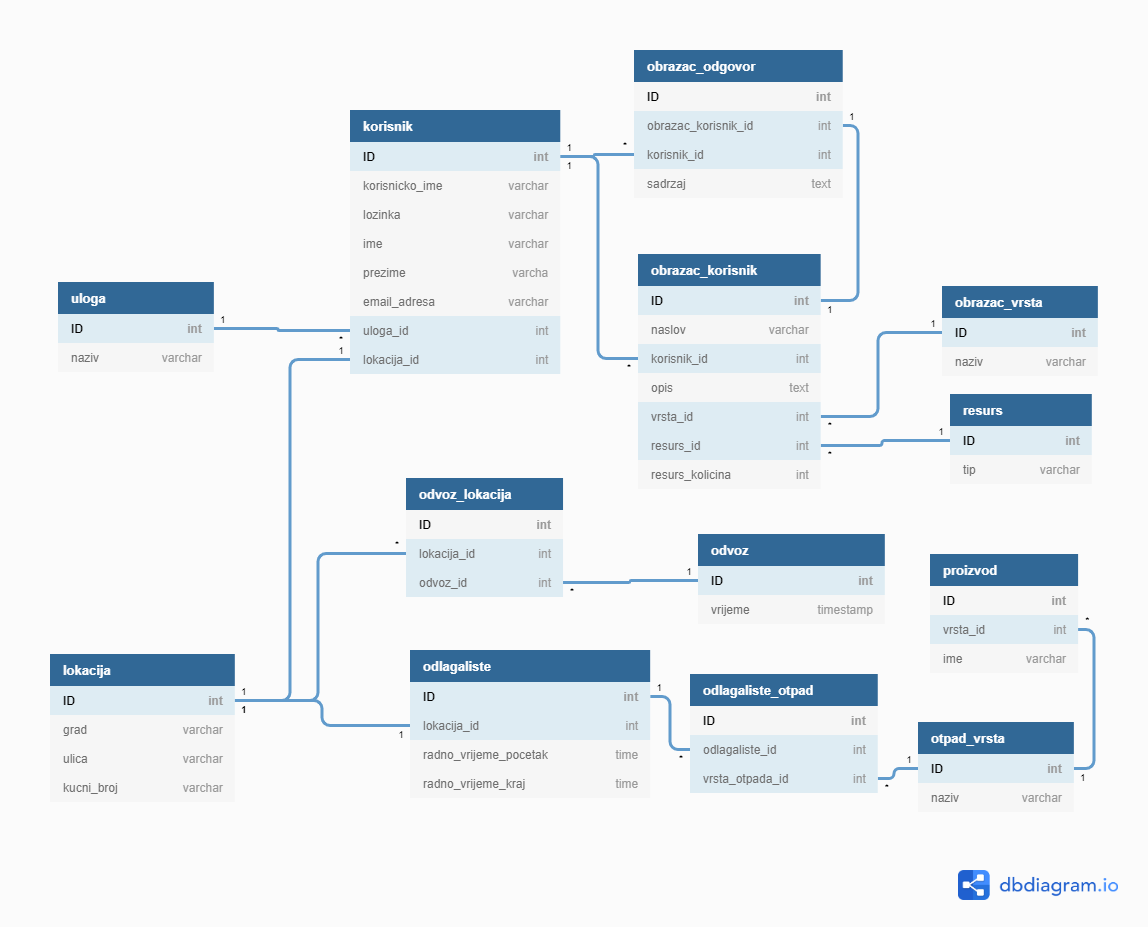
\includegraphics[width=\textwidth]{slike/baza_podataka.png}
					
					\caption{Baza podataka}
					\label{fig:baza_podataka}
				\end{figure}
			
			\eject
		\clearpage	
			
		\section{Dijagram razreda}
		Dijagram razreda prikazuje odnose asocijacije i agregacije između razreda u našoj aplikaciji.Dijagram je modeliran

		prema opisu baze tako da brojnost odgovara modelu baze.Korisnik je apstraktni razred kojeg nasljeđuju građanin,zaposlenik i administrator u implementaciji aplikacije.Za slanje obrazaca su vezani razredi ObrazacOdgovor i Korisnikov obrazac koji prema enumeraciji može biti zahtjev za resursima,zahtjev za glomaznim otpadom ili pritužba.Razred Lokacija je povezan sa građaninom (boravište) i odlagalištem.Razred Odvoz ukazuje na mogućnost odvoza na određenim lokacijama, dok odlagališta mogu sakupljati različite vrste otpadnih proizovda.

		
			\begin{figure}[H]
				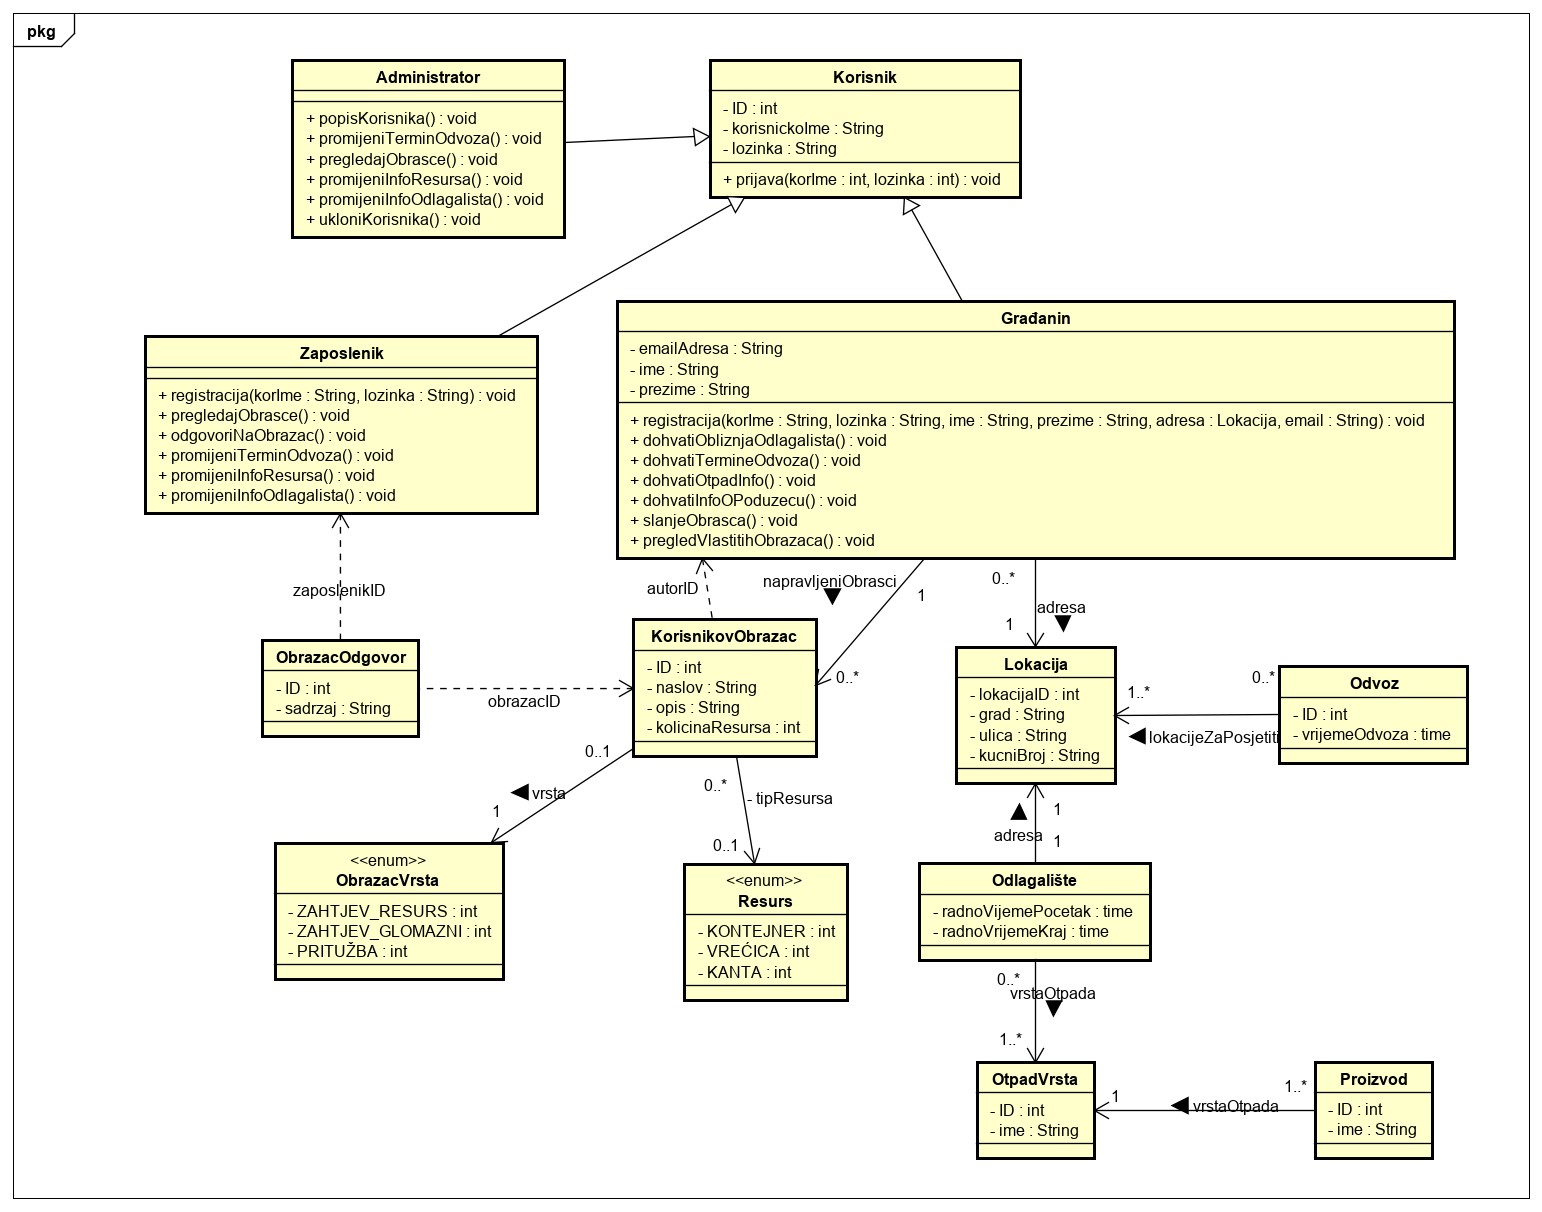
\includegraphics[width=\linewidth]{dijagrami/Dijagram razreda.png}
				\centering
				\caption{Dijagram razreda}
				\label{fig:dijagram_razreda}
			\end{figure}
			
			
			\eject
			\clearpage
			
		\section{Implementacijski dijagram razreda}
		
		Zbog kompleksnosti dijagrama, on će biti podijeljen na nekoliko njih po slojevima.
		
		\subsection{Sloj domene}
		\begin{figure}[H]
			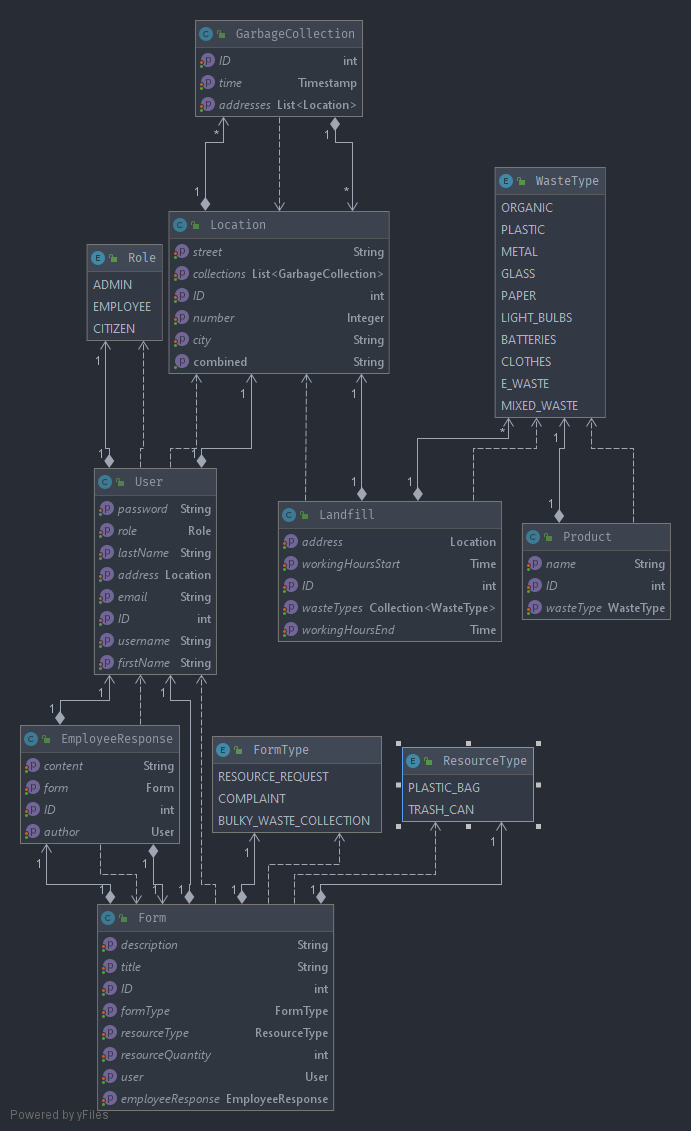
\includegraphics[width=0.7\linewidth]{slike/modelSloj.png}
			\centering
			\caption{Sloj domene}
			\label{fig:sloj_domene}
		\end{figure}
	
		\subsection{Sloj za pristup podacima }
		\begin{figure}[H]
			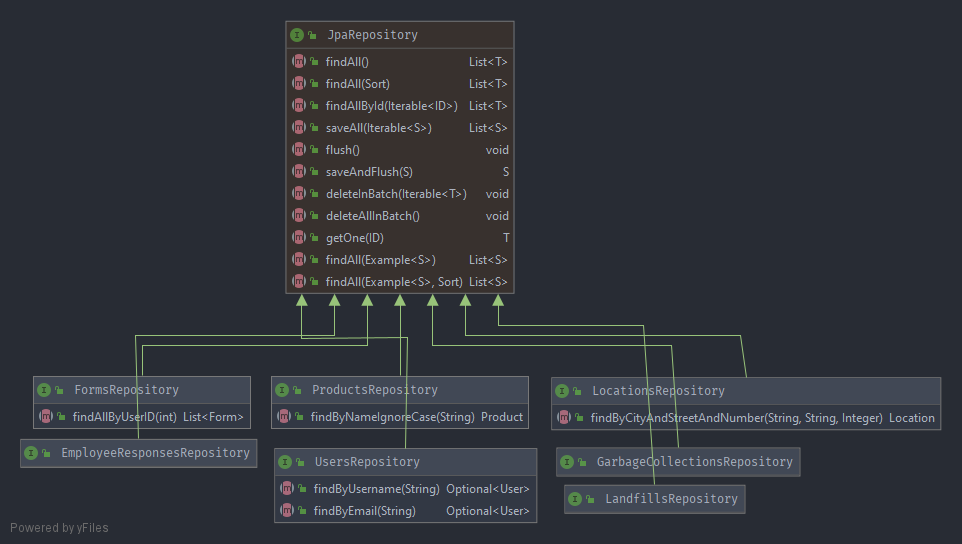
\includegraphics[width=\linewidth]{slike/daoSloj.png}
			\centering
			\caption{Sloj za pristup podacima}
			\label{fig:dao_sloj}
		\end{figure}
	
		\subsection{Sloj usluge}
		\begin{figure}[H]
			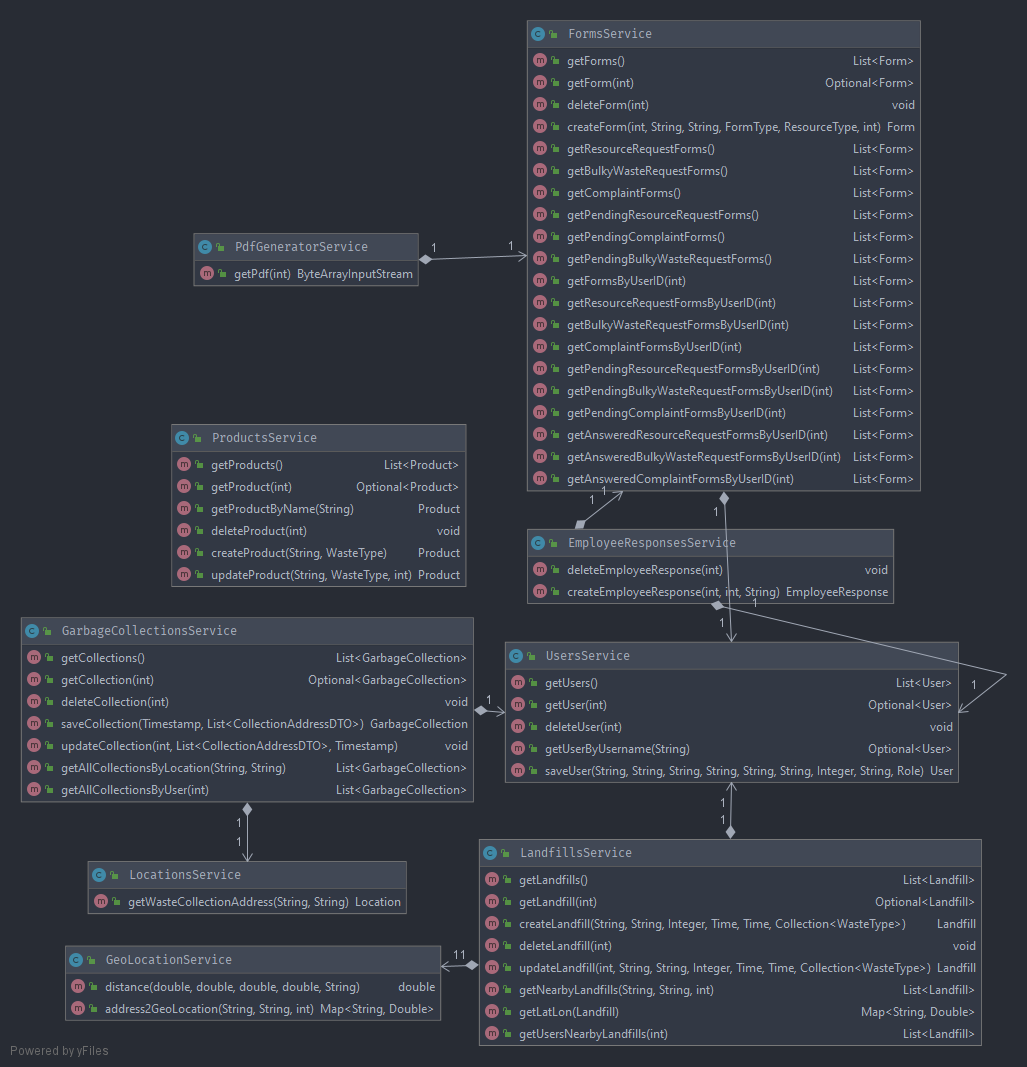
\includegraphics[width=\linewidth]{slike/serviceSloj.png}
			\centering
			\caption{Sloj usluge}
			\label{fig:service_sloj}
		\end{figure}
	
		\subsection{Sloj nadglednika}
		\begin{figure}[H]
			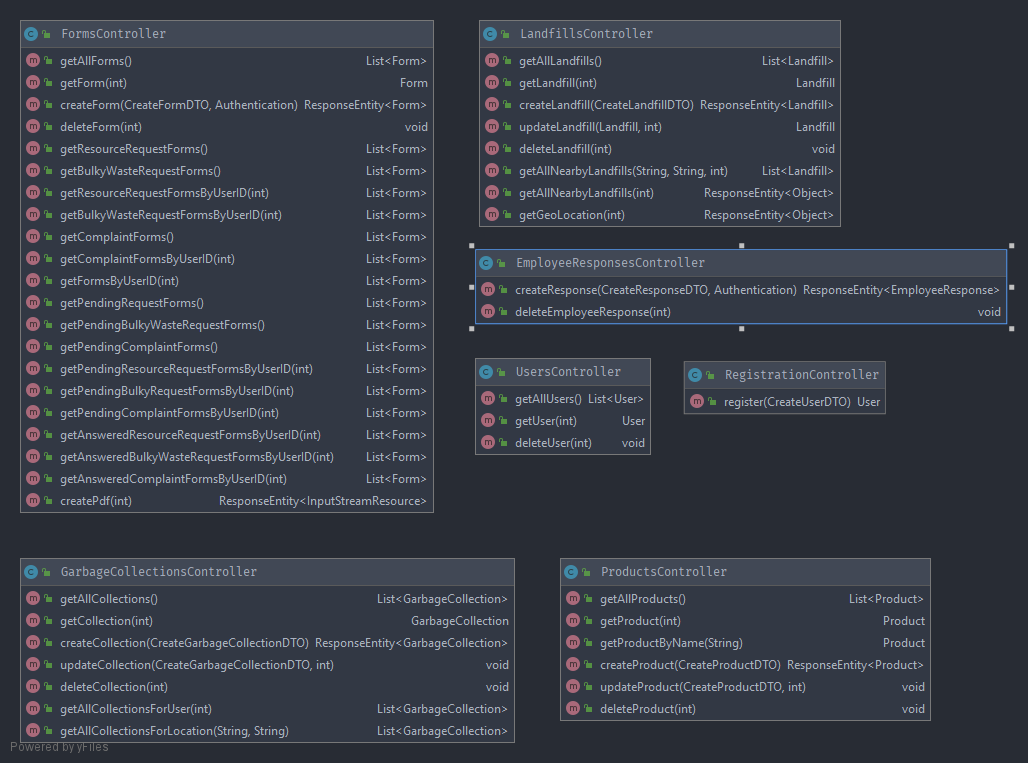
\includegraphics[width=\linewidth]{slike/controllersSloj.png}
			\centering
			\caption{Sloj nadglednika}
			\label{fig:controller_sloj}
		\end{figure}
		
		\subsection{DTO razredi}
		\begin{figure}[H]
			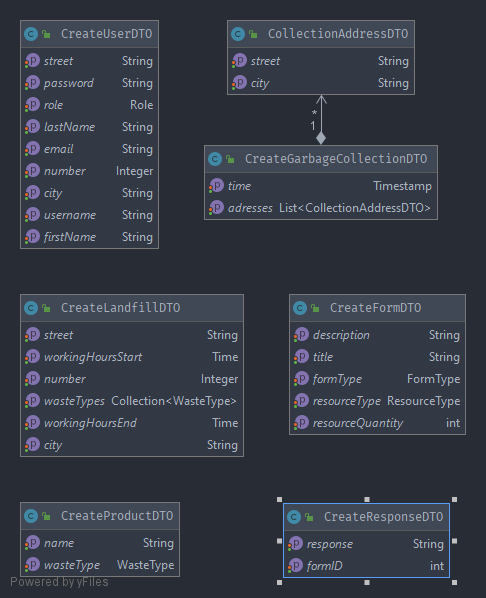
\includegraphics[width=0.7\linewidth]{slike/dtos.png}
			\centering
			\caption{DTO razredi}
			\label{fig:dtos}
		\end{figure}
	
		\subsection{REST dijagram (Controller + DTO + Service)}
		\begin{figure}[H]
			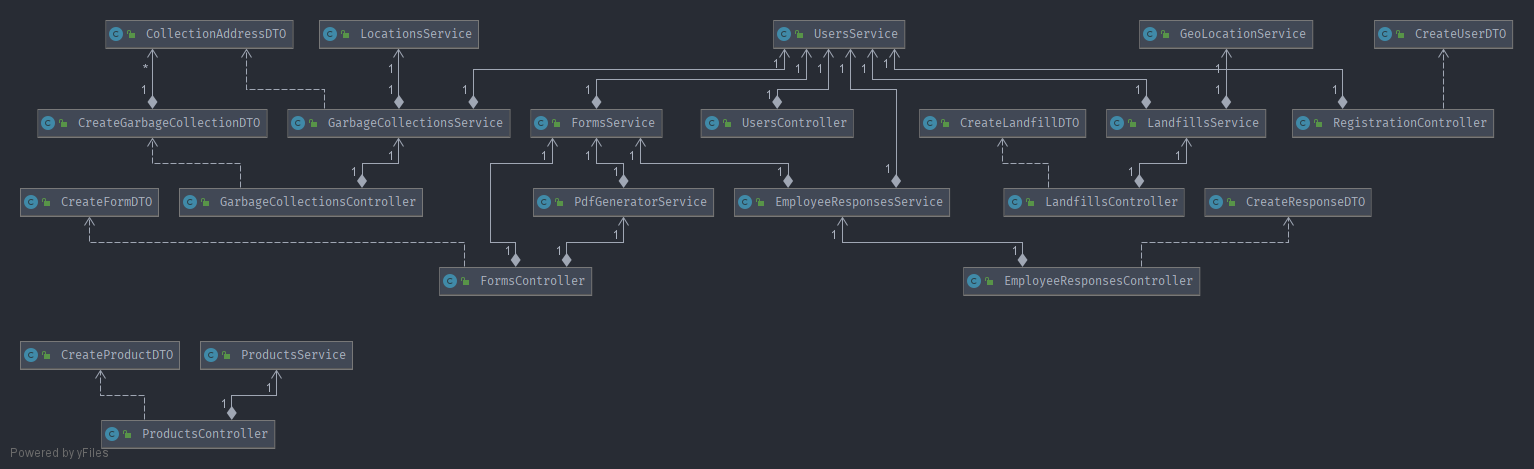
\includegraphics[width=\linewidth]{slike/REST_ControllerDTOService.png}
			\centering
			\caption{REST dijagram}
			\label{fig:rest_razredi}
		\end{figure}
		
				
		\clearpage
		

		\section{Dijagram stanja}
		
%			\textbf{\textit{dio 2. revizije}}\\
%			
%			\textit{Potrebno je priložiti dijagram stanja i opisati ga. Dovoljan je jedan dijagram stanja koji prikazuje \textbf{značajan dio funkcionalnosti} sustava. Na primjer, stanja korisničkog sučelja i tijek korištenja neke ključne funkcionalnosti jesu značajan dio sustava, a registracija i prijava nisu. }
%			
		Pomoću dijagrama stanja možemo prikazati prijelaze iz jednog stanja u drugo ovisno o događaju. Na slikama su prikazani takvi dijagrami. Nakon prijave zaposlenik se nalazi na početnoj stranici na kojoj može vidjeti osnovne informacije o poduzeću. Daljnjim odabirom može odabrati želi li otići na stranicu za "Zahtjeve i pritužbe" ili "dodatne Informacije" gdje mu se nude dodatne opcije. Kod "Zahtjeva i pritužbi" može odabrati "Dodatne resurse" i tamo klikom na "Odgovori" odgovoriti na trenutne zahtjeve ili klikom na "Obriši" obrisati zahtjev. Osim u stanju "Dodatni resursi" zaposlenik može raditi iste događaje i u stanjima  "Glomazni otpad" i "Pritužbe". Kod stanja za informacije može se izabrati kakve dodatne informacije želi vidjeti. U stanju "odgovarajuće odlagalište za traženi proizvod" može uređivati taj proizvod znači mijenjati mu ime ili tip resursa, prikazati mjesto odlaganju toga proizvoda, ali i brisati i dodavati. Kod pregleda odlagališta može vidjeti lokacije trenutnih odlagališta i dodati novo odlagalište. U stanju Termini odvoza otpada prikazuju mu se svi termini koji su uneseni, a nadalje može još dodavati, brisati i pregledavati po lokaciji te termine.
		\begin{figure}[H]
			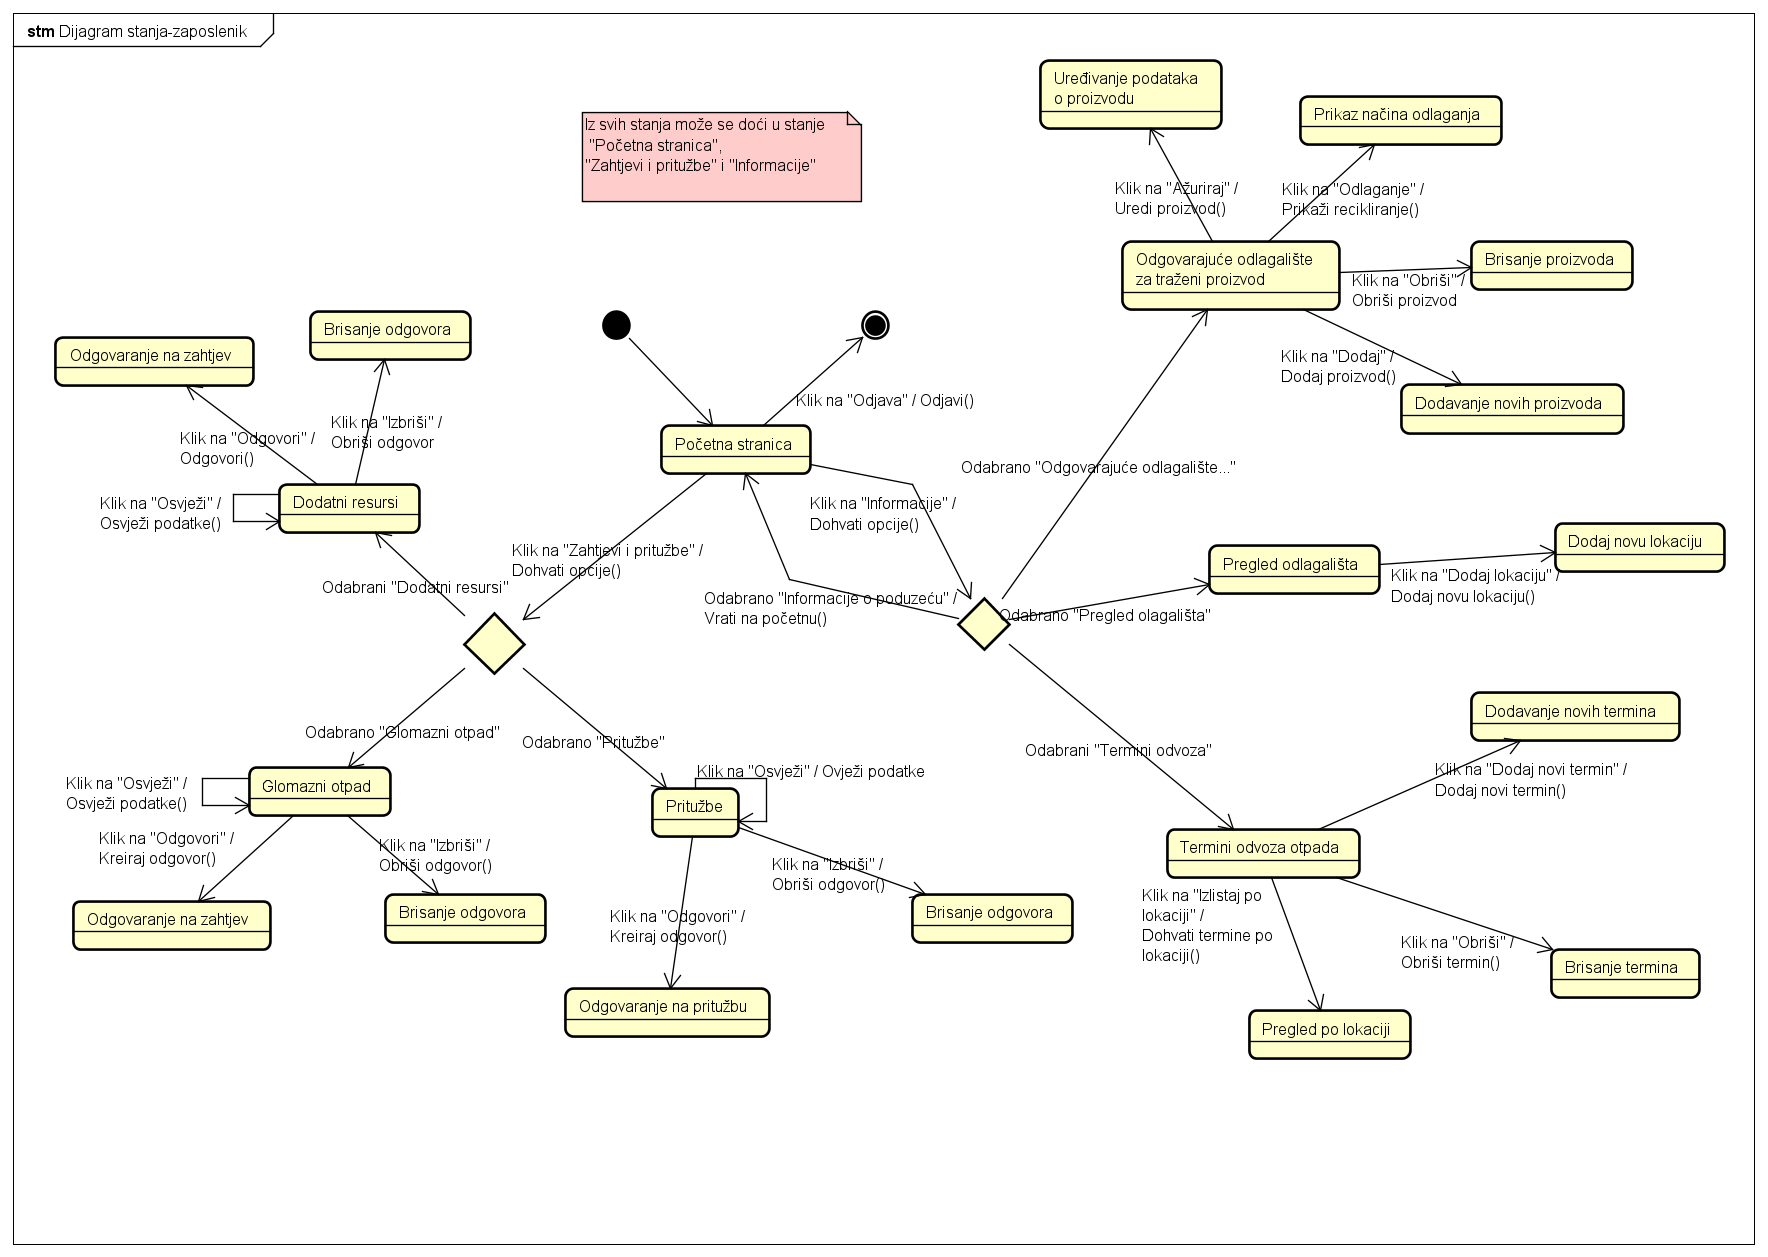
\includegraphics[width=\linewidth]{dijagrami/Dijagram stanja-zaposlenik.png}
			\centering
			\caption{Dijagram stanja-zaposlenik}
			\label{fig:dijagram_stanja-zaposlenik}
		\end{figure}
	
		Za građanina dijagram je sličan samo što građanin nema opcije brisanja i dodavanja novih termina i lokacija, ali ima iste mogućnosti pregledavanja tih termina i lokacija. Osim pregledavanja korisnik može kada se nalazi u stanju "Dodatni resursi" zatražiti dodatne resurse klikom na "Novi zahtjev" gdje mu se otvara novi prostor za unos detalja o zahtjevi. Iste događaje može napraviti kada se nalazi i u stanju "Glomazni otpad" i "Moje pritužbe".
		\begin{figure}[H]
			\includegraphics[width=\linewidth]{dijagrami/Dijagram stanja-građanin.png}
			\centering
			\caption{Dijagram stanja-građanin}
			\label{fig:dijagram_stanja-građanin}
		\end{figure}
%			
			\eject 
%		
		\section{Dijagram aktivnosti}
			
%			\textbf{\textit{dio 2. revizije}}\\                                                                                                                                                                               7
			
			 Dijagram aktivnosti služi za opis modela toka upravljanja ili toka podataka. Inicijalno stanje označeno je crnim kružićem, dok je završno stanje prikazano zaokruženim crnim kružićem. Na dijagramu aktivnosti 4.6 prikazan je proces kreiranja zahtjeva za glomaznim otpadom. Korisnik se najprije prijavljuje u sustav, te ako su njegovi podaci točni, prosljeđuje ga se na početnu stranicu web aplikacije. Nakon toga korisnik odabire zahtjev za odvoz glomaznog otpada te može generirati vlastiti zahtjev ukoliko ne postoji nikakav neodgovoreni zahtjev. Slična implementacija funkcionira za slanje pritužbi te za slanje zahtjeva za dodatnim resursima.
			 
			 
			 \begin{figure}[H]
			 	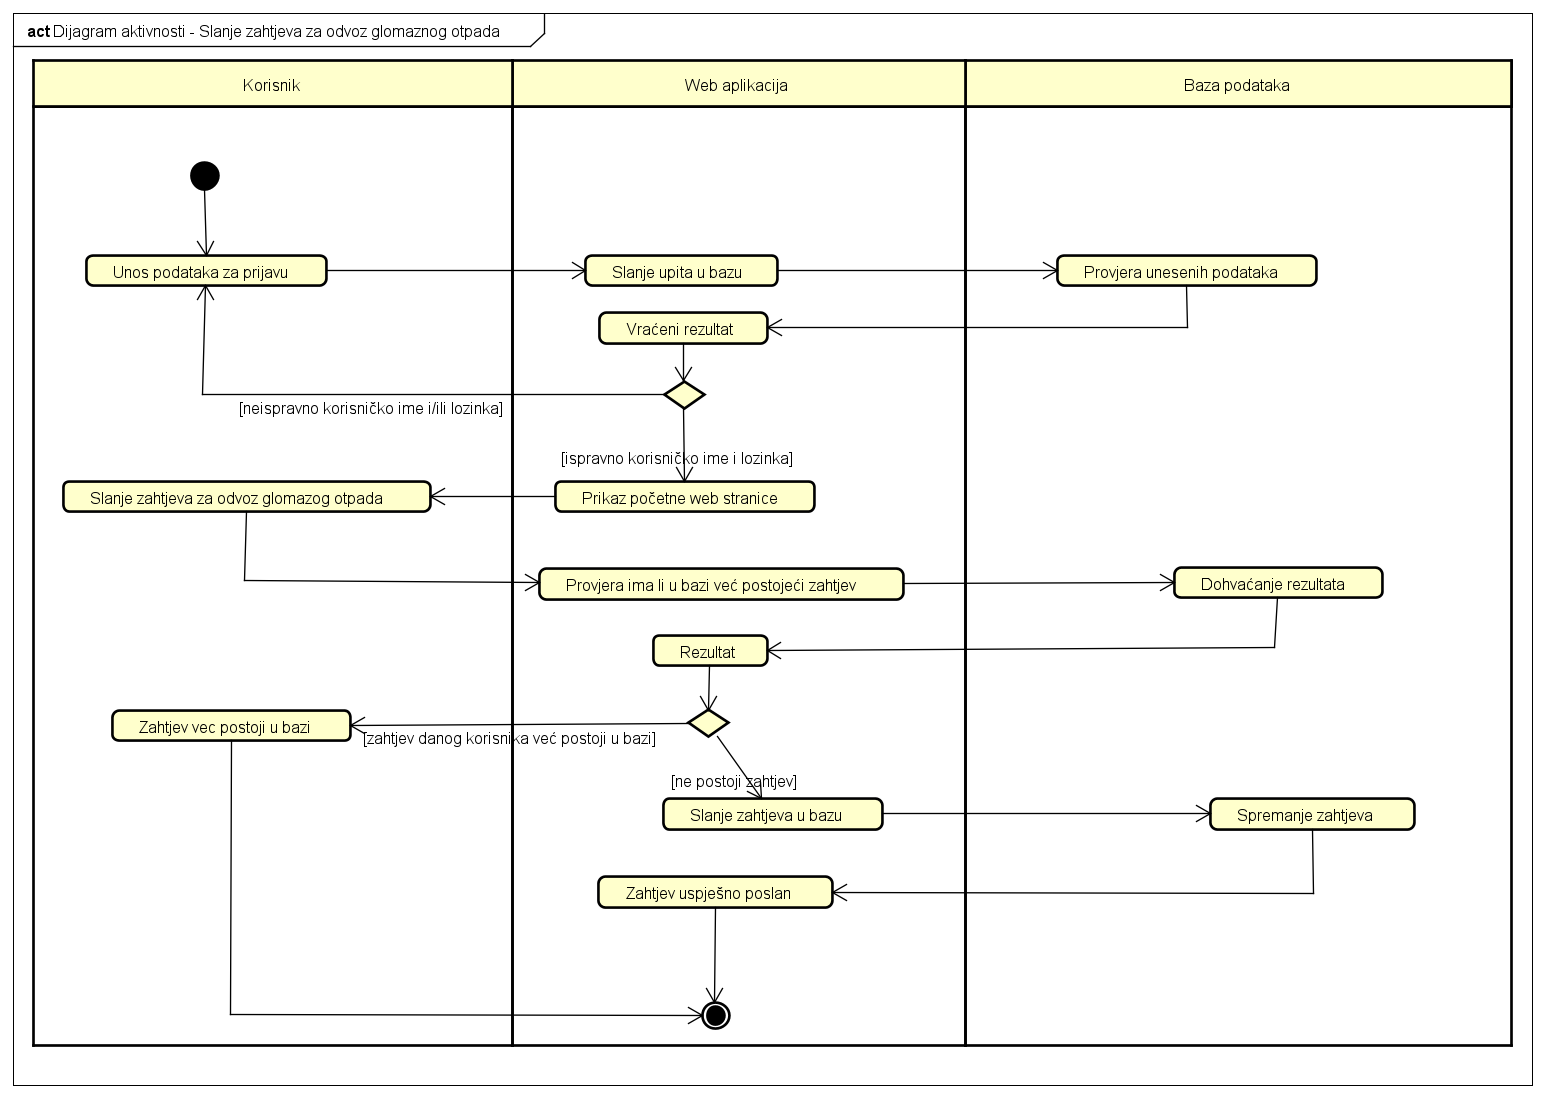
\includegraphics[width=\linewidth]{dijagrami/Dijagram aktivnosti.png}
			 	\centering
			 	\caption{Dijagram aktivnosti}
			 	\label{fig:dijagram_aktivnosti}
			 \end{figure}
			 
			
			\eject
		\clearpage
		
		\section{Dijagram komponenti}
		
%			\textbf{\textit{dio 2. revizije}}\\
			 Dijagram komponenti koristi se za prikaz međuovisnosti komponenata, internu strukturu te odnose prema okolini. Sustav koristi dva sučelja. Sa sučeljem dohvat HTML, CSS i JS datoteka dohvaća se frontend dio aplikacije. Komponenta koja opslužuje HTML, CSS i JS datoteke je router koji zna koju datoteku opslužiti pomoću zahtjeva s url-om. Routerom se može doći do datoteka za prijavu, registraciju i početnih stranica određenih aktora. Biblioteke koje se uključuju u datoteke frontend dio aplikacije su react, bootstrap za ukrašene komponente i leaflet za karte. 
			 Sučeljem za dohvat JSON podataka pristupa se REST API komponenti. REST API prihvaća sve podatke i
			 poziva odgovarajuće metode za prihvat u Controllers komponenti. Jpa Repositories zadužen je za 
			 dohvaćanje tablica iz baze podataka. Pretvara podatke u DAO modele i šalje ih ostatku backend
			 aplikacije (Service sloju). Controllers komponenta obrađuje pristigle upite iz REST API komponente
			 i poziva odgovarajuće metode iz Service sloja. Service sloj zadužen je za usluge koje se obavljaju nad
			 podatcima iz baze podataka koji su mapirani u komponenti Models.
			 
			 \begin{figure}[H]
			 	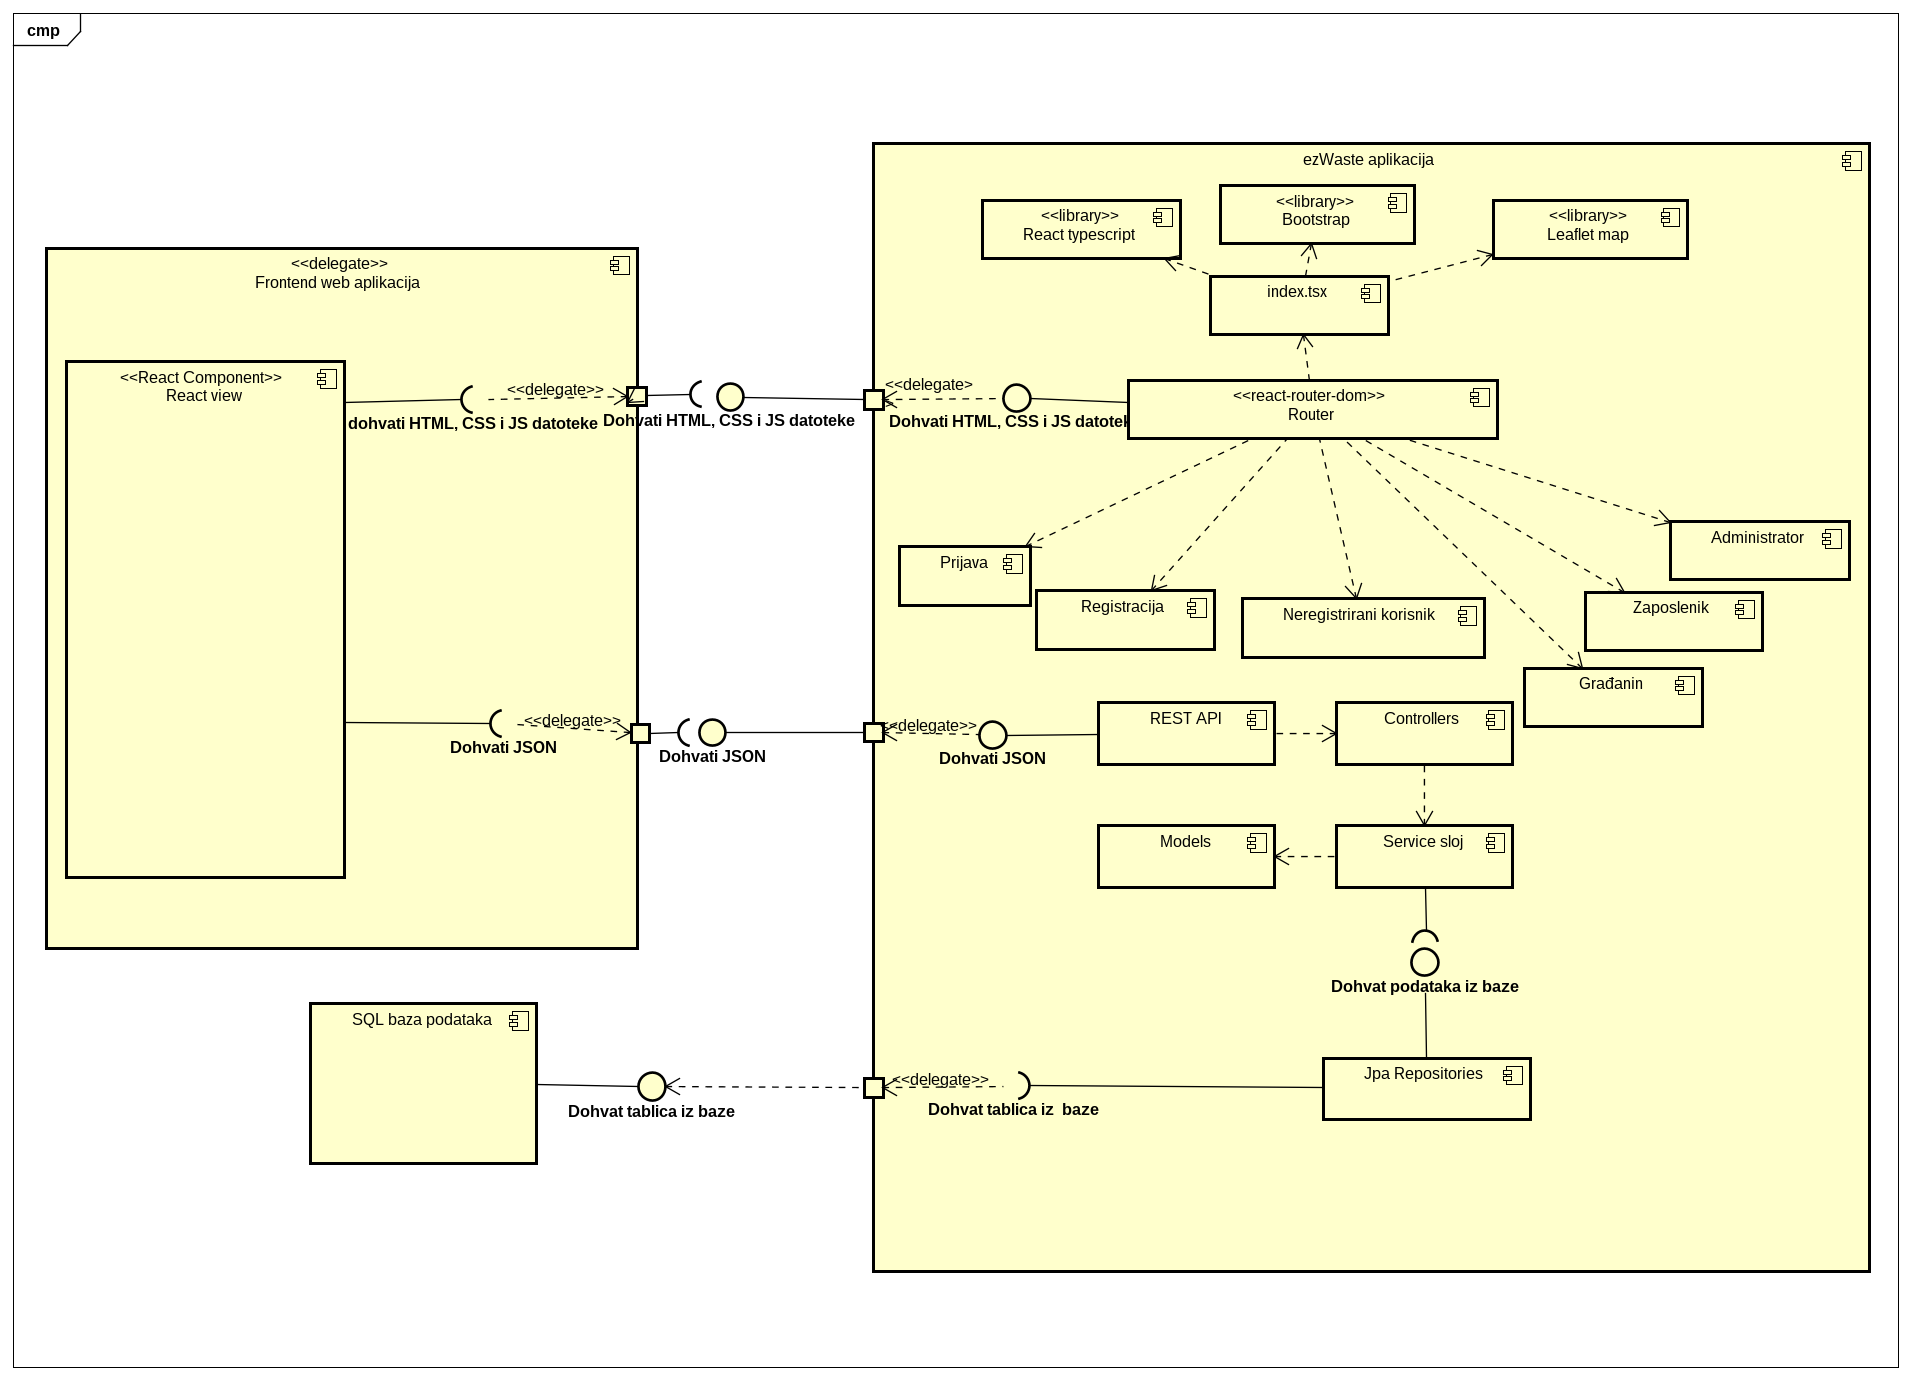
\includegraphics[width=\linewidth]{dijagrami/Dijagram komponenti.png}
			 	\centering
			 	\caption{Dijagram komponenti}
			 	\label{fig:dijagram_komponenti}
			 \end{figure}
			 
			 
			 \eject
